\documentclass[9pt, a4paper, oneside]{article} % Paper size, default font size and one-sided paper
%\graphicspath{{./Figures/}} % Specifies the directory where pictures are stored
%\usepackage[dcucite]{harvard}
\usepackage{rotating}
\usepackage{amsmath}
\usepackage{setspace}
\usepackage{pdflscape}
\usepackage[flushleft]{threeparttable}
\usepackage{multirow}
\usepackage{tikz}
\usepackage[comma, sort&compress]{natbib}% Use the natbib reference package - read up on this to edit the reference style; if you want text (e.g. Smith et al., 2012) for the in-text references (instead of numbers), remove 'numbers' 
\usepackage{graphicx}
%\bibliographystyle{plainnat}
\bibliographystyle{agsm}
\usepackage[colorlinks = true, citecolor = blue, linkcolor = blue]{hyperref}
%\hypersetup{urlcolor=blue, colorlinks=true} % Colors hyperlinks in blue - change to black if annoying
%\renewcommand[\harvardurl]{URL: \url}
 \usepackage{listings}
 \usepackage{color}
\definecolor{mygrey}{gray}{0.95}
\lstset{backgroundcolor=\color{mygrey}}
\begin{document}
\title{MSc Finance Structure}
%\author{Rob Hayward\footnote{University of Brighton Business School, Lewes Road, Brighton, BN2 4AT; Telephone 01273 642586.  rh49@brighton.ac.uk}}
%\date{\today}
%\maketitle
\section*{MSc Finance Meeting}

Thanks to everyone for coming along yesterday.  I think that the main points were:

\begin{itemize}
\item We will create a \emph{research methods} module that will support the dissertation and provide key skills for employability
\item We will add some pathways that will probably include MSc Finance and Accounting, MSc Economics and Banking and MSc Finance and Risk Management. 
\item We will update the existing core module specification and rationalise the elective menu.
\end{itemize}

There was a discussion about block teaching of electives. This will begin this year with a pattern of three day delivery around the weekend (Thursday, Friday, Monday or Friday, Monday, Tuesday).  This will avoid some of the problems that we have faced with the timing of Easter and the limited time between the end of the modules and the exam period. 

There was a discussion of the proposed new research methods module.  Most thought that this should be rooted in practice to be most effective and that it should be combined with the teaching of the quantitative techniques and that these techniques should also be aligned with the teaching in the finance and economics modules.  

Ray Bachan and Pascal Stiefenhofer will produce a module specification for the new research methods module.  Andros Gregoriou, Jerome Healy, Jairaj Gupta and Marc Blunden will update the finance module specification.  Sushil Mohan, Ray Bachan and Rob Hayward will update the economics module.  

This is one structure for the course that was discussed. Here Phase One economics and finance are merged into their Phase Two partners and the Research Methods includes appropriate quantitative techniques.  

\begin{figure}[h]
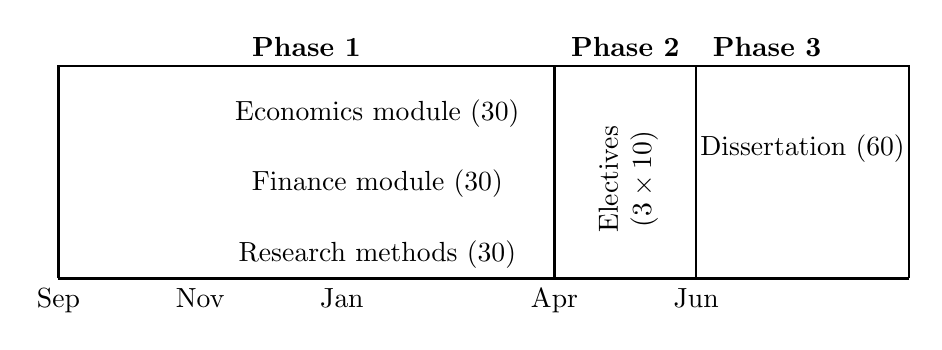
\begin{tikzpicture}[scale = 0.9]
%\draw [help lines] (0, 0) grid (12, 3);
\node [below] at (0, 0) {Sep};
\node [below] at (2, 0) {Nov};
\node [below] at (4, 0) {Jan};
\node [below] at (7, 0) {Apr};
\node [below] at (9, 0) {Jun};
\draw [very thick] (0, 0) -- (12, 0);
\draw [thick] (0,0) -- (0, 3) -- (7, 3) -- (7, 0);
\node [above] at (3.5, 3) {\textbf{Phase 1}};
%\node [above] at (3.5, 2) {ECM02};
%\node [above] at (3.5, 1) {FN};
%\node [above] at (3,5, 0) {OP394}; 
%\draw [thick] (2,0) -- (2, 3) -- (7, 3) -- (7, 0);
%\node [above] at (4.5, 3) {\textbf{Phase 2}};
\node [above] at (4.5, 2) {Economics module (30)};
\node [above] at (4.5, 1) {Finance module (30)};
\node [above] at (4.5, 0) {Research methods (30)};
\draw [thick] (7,0) -- (7, 3) -- (9, 3) -- (9, 0);
\node [above] at (8, 3) {\textbf{Phase 2}};
\node [above, rotate = 90, align = center] at (8.6, 1.4) {Electives\\($3\times10$)};
\draw [thick] (9,0) -- (9, 3) -- (12, 3) -- (12, 0);
\node [above] at (10, 3) {\textbf{Phase 3}};
\node [above] at (10.5, 1.5) {Dissertation (60)};
\end{tikzpicture}
\end{figure}
There was some argument for maintaining 20 and 10 CAT modules and some suggestion that they be augmented by some supportive block teaching at the beginning of the academic year. 

\section*{To be done}

\begin{itemize}
\item We will begin by considering the core content of the key economics and finance modules and mapping the quantitative skills that can be provided in the new research methods.  Let's have another meeting before the end of the year to take a look at that.  
\item New electives will have to be created to support the pathways.  That would include banking, managerial economics, risk management and some accounting modules. 
\item All existing module specifications will have to be updated using the latest template at some point. 
\end{itemize}


\end{document}
